\documentclass[a4paper]{article}

\usepackage{../inc/ssarticle}

\title{{\centering\huge {Agentes auto-propulsados: Boids}}}

\begin{document}
\begin{titlingpage}
    \maketitle
    \begin{abstract}
        En el presente informe, se realiza un estudio del comportamiento de bandadas de agentes autopropulsados mediante la implementación y análisis del paper propuesto por Reynolds, C. W. \cite{BoidsPaper}.
    \end{abstract}
\end{titlingpage}

    \tableofcontents
    \newpage

    \section{Fundamentos}
        \subsection{Boids}
            Reynolds propuso un modelo para simular bandadas de agentes que se basa en la aplicación a cada uno de los agentes una lista determinada de reglas. Las mismas terminan influenciando como es que cada agente se mueve y como interactua con lo que lo rodea.

            A alto nivel, el funcionamiento del algoritmo es el siguiente:

            \begin{algorithm}
                \caption{Boids}\label{pseudo:boids}
                \begin{algorithmic}[1]
                    \Procedure{Step}{$rules, factors, boids, dT$}
                    \For{$boid \gets boids$}
                        \State $\bm{v} = boid.velocity$
                        \For{$rule \gets rules$}
                            \State $\bm{v} \mathrel{+}= factor_i * rule(boid, boids)$
                        \EndFor
                        \If{$magnitude(\bm{v}) > MAX\_SPEED$}
                            \State $\bm{v} = \bm{v} / magnitude(\bm{v}) * MAX\_SPEED$
                        \EndIf
                        \State $boid.velocity = v$
                        \State $boid.position \mathrel{+}= boid.velocity * dT$
                    \EndFor
                \EndProcedure
                \end{algorithmic}
            \end{algorithm}

            A cada una de las reglas se la multiplica por un factor, para hacer que su influencia sobre el sistema sea mayor o menor.

            \subsubsection{Vecinos}
            Dado que todas las reglas son de interacción entre \textit{boids}, se define un radio $distance$ y un ángulo $angle$ dentro del cual deben de estar los otros \textit{boids} para ser considerados vecinos:

            \begin{figure}[H]
                \centering
                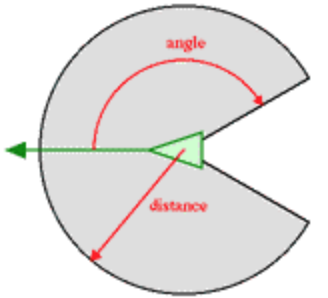
\includegraphics[width=0.25\textwidth]{{../imgs/neighbourhood}.png}
                \caption{Vecinos}
                \label{fig:neighbourhood}
            \end{figure}

            \subsubsection{Reglas básicas}

            Reynolds propone tres reglas básicas para poder generar un comportamiento de bandada.

            Unicamente los \textit{boids} que están dentro del círculo afectan al \textit{boid}.

            \begin{center}
                \begin{table}[h]
                    \begin{tabular}{ccc}
                        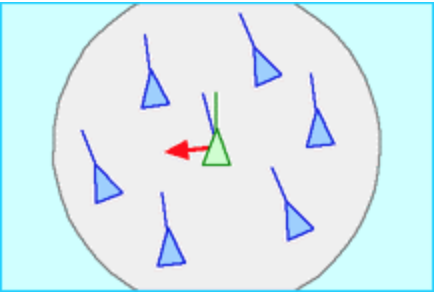
\includegraphics[width=0.25\linewidth]{{../imgs/rule_alignment}.png} &
                        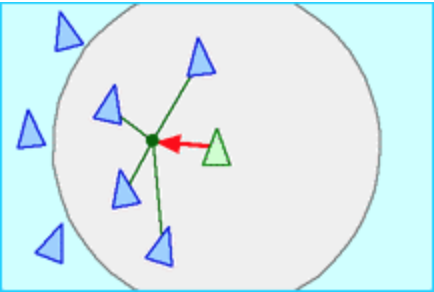
\includegraphics[width=0.25\linewidth]{{../imgs/rule_cohesion}.png} &
                        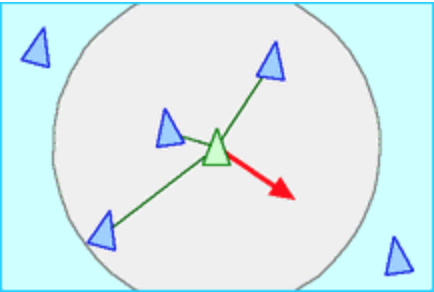
\includegraphics[width=0.25\linewidth]{{../imgs/rule_separation}.png} \\
                        Alineamiento & Cohesión & Separación \\
                    \end{tabular}
                    \end{table}
            \end{center}

            La regla de \textbf{alineamiento} hace que cada \textit{boid} busque alinearse con los vecinos:

            \begin{algorithm}
                \caption{Alineamiento}\label{pseudo:alignment}
                \begin{algorithmic}[1]
                    \Procedure{Alineamiento}{$boid, boids$}
                    \State $\bm{v}_{out} = \{0, 0, 0\}$
                    \For{$neighbour \gets boids$}
                        \State $\bm{v}_{out} \mathrel{+}= neighbour.velocity$
                    \EndFor
                    \State $\bm{v}_{out} = \bm{v}_{out} / length(neighbours)$\Comment{Velocidad promedio de vecinos}
                    \State $\bm{v}_{out} = \bm{v}_{out} - boid.velocity$
                    \State \textbf{return} $\bm{v}_{out}$
                    \EndProcedure
                \end{algorithmic}
            \end{algorithm}

            La regla de \textbf{cohesión} hace que cada \textit{boid} busque moverse hacia el \textit{centro de masa} de la bandada, siendo el \textit{centro de masa}, la posición promedio de los vecinos:

            \begin{algorithm}
                \caption{Cohesión}\label{pseudo:cohesion}
                \begin{algorithmic}[1]
                    \Procedure{Cohesión}{$boid, boids$}
                    \State $\bm{v}_{out} = \{0, 0, 0\}$
                    \For{$neighbour \gets boids$}
                        \State $\bm{v}_{out} \mathrel{+}= neighbour.position$
                    \EndFor
                    \State $\bm{v}_{out} = \bm{v}_{out} / length(neighbours)$\Comment{Posición promedio de vecinos}
                    \State $\bm{v}_{out} = \bm{v}_{out} - boid.position$
                    \State \textbf{return} $\bm{v}_{out}$
                    \EndProcedure
                \end{algorithmic}
            \end{algorithm}

            La regla de \textbf{separación} hace que cada \textit{boid} busque estar a una cierta distancia de cada uno de sus vecinos. A diferencia de las reglas anteriores, un boid es considerado vecino si está a una distancia menor que la distancia de interacción que se aplica para el resto de las reglas:

            \begin{algorithm}
                \caption{Separación}\label{pseudo:separation}
                \begin{algorithmic}[1]
                    \Procedure{Separación}{$boid, boids$}
                    \State $\bm{v}_{out} = \{0, 0, 0\}$
                    \For{$neighbour \gets boids$}
                        \If{$distance(neighbour, boid) > unsafeDistance$}
                            \State \textbf{continue}
                        \EndIf
                        \State $\bm{v}_{out} \mathrel{-}= boid.position - neighbour.position$
                    \EndFor
                    \State $\bm{v}_{out} = \bm{v}_{out} / length(neighbours)$\Comment{Posición promedio de vecinos}
                    \State $\bm{v}_{out} = \bm{v}_{out} - boid.position$
                    \State \textbf{return} $\bm{v}_{out}$
                    \EndProcedure
                \end{algorithmic}
            \end{algorithm}

            \pagebreak
            \subsubsection{Reglas extendidas}
                A demás de las reglas básicas, en el trabajo se implementaron un conjunto de reglas extras que buscan agregar complejidad al sistema.

                La regla \textbf{TendencyTo} es una regla que puede interpretarse de dos maneras dependiendo del factor que se le aplique. Un factor positivo hace que las entidades se acerquen a otras de un tipo específico, mientras que un factor negativo hace que se alejen:

                \begin{algorithm}
                    \caption{TendencyTo}\label{pseudo:tendency_to}
                    \begin{algorithmic}[1]
                        \Procedure{TendencyTo}{$boid, neighbours, interactWith$}
                            \State $\bm{v}_{out} = \{0, 0, 0\}$
                            \For{$neighbour \gets neighbours$}
                                \If{$neighbour.type \mathrel{!}= interactWith$}
                                    \State \textbf{continue}
                                \EndIf
                                \State $\bm{v}_{out} \mathrel{+}= (neighbour.position - boid.position) / 10$
                            \EndFor
                        \EndProcedure
                    \end{algorithmic}
                \end{algorithm}

                La regla \textbf{Boundary} busca hacer que si un \textit{boid} se escapa del universo sin condiciones de contorno, el mismo vuelva de una manera "orgánica" sin tener saltos abruptos en la velocidad:

                \pagebreak

                \begin{algorithm}
                    \caption{Boundary}\label{pseudo:boundary}
                    \begin{algorithmic}[1]
                        \Procedure{Boundary}{$boid, universe$}
                            \State $x_{min} \gets universe.metadata.boundaries.minx$
                            \State $x_{max} \gets universe.metadata.boundaries.maxx$
                            \State $y_{min} \gets universe.metadata.boundaries.miny$
                            \State $y_{max} \gets universe.metadata.boundaries.maxy$
                            \State $z_{min} \gets universe.metadata.boundaries.minz$
                            \State $z_{max} \gets universe.metadata.boundaries.maxz$
                            \State $speed \gets CONST$
                            \State $\bm{v} \gets \{0, 0, 0\}$
                            \If{$boid.x < x_{min}$}
                                \State $\bm{v}_x = speed$
                            \EndIf
                            \If{$boid.x > x_{max}$}
                                \State $\bm{v}_x = -speed$
                            \EndIf
                            \If{$boid.y < y_{min}$}
                                \State $\bm{v}_y = speed$
                            \EndIf
                            \If{$boid.y > y_{max}$}
                                \State $\bm{v}_y = -speed$
                            \EndIf
                            \If{$boid.z < z_{min}$}
                                \State $\bm{v}_z = speed$
                            \EndIf
                            \If{$boid.z > z_{max}$}
                                \State $\bm{v}_z = -speed$
                            \EndIf
                            \State \textbf{return} $\bm{v}$
                        \EndProcedure
                    \end{algorithmic}
                \end{algorithm}

        \subsection{Polarización}
            Polarización es un parámetro que permite tener un indicador sobre el estado de alineamiento de las velocidades de los \textit{boids} dentro del universo (ignorando los depredadores). La misma adquiere valores entre $0$ (desorden, cada \textit{boid} se mueve en una dirección distinta al resto) y $1$ (orden, todos los \textit{boids} se mueven en la misma dirección).

            Para definir polarización en tres dimensiones se sigue el modelo propuesto por \textit{Vicsek et al.}\cite{PhysRevLett.75.1226} ya que aplica de igual manera para dos que para tres dimensiones. Se modifica el denominador $Nv$ ya que cada \textit{boid} tiene su propia rapidez:

            $$v_{avg} = \frac{\sum_{i=1}^{N}\left|\mathbf{v}_i\right|}{N}$$
            $$v_a = \frac{1}{v_{avg}}\left|\sum_{i=1}^{N}\mathbf{v}_i\right|$$

            donde $N$ es la cantidad de agentes en el universo y $\mathbf{v}_i$ es la velocidad de cada agente.

    \section{Implementación}

        \subsection{Universo}

            El universo utilizado para realizar la simulación es un hiperrectánculo con un largo $W$, alto $H$ y profundidad $D$. Es posible crear simulaciones con o sin condiciones de contorno.

            Una vez creado, el universo no puede ser modificado (ni sus dimensiones, ni parámetros, ni entidades), por lo que al avanzar la simulación equivale a crear fotos del universo para cada tiempo específico.


            \begin{figure}[H]
                \centering
                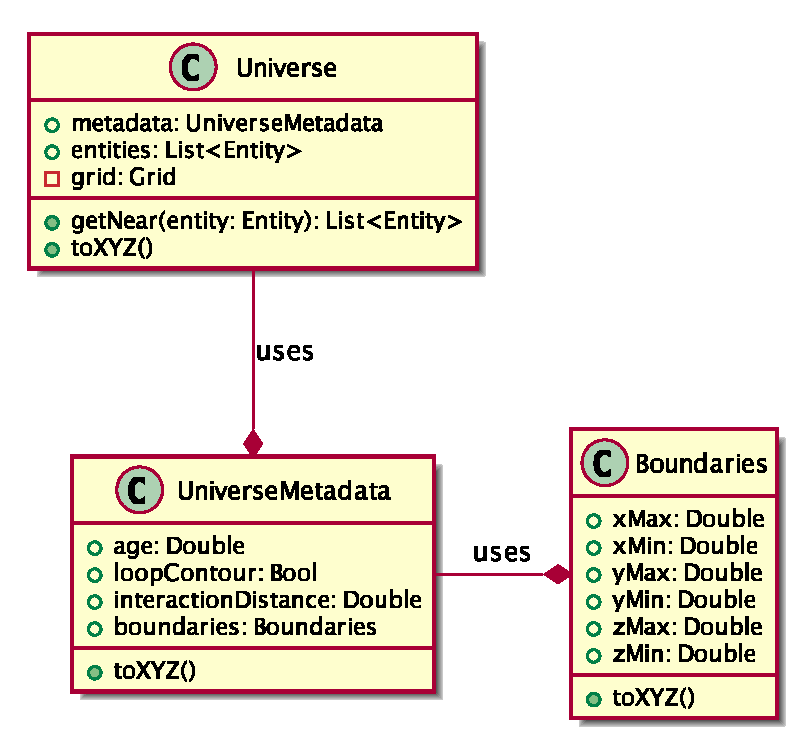
\includegraphics[width=0.5\textwidth]{../imgs/universe}
                \caption{Universo}
                \label{fig:universe_implementation}
            \end{figure}

        \subsection{Grilla}

            \textit{Grid} es la implementación de \textit{Cell index method}. \\
            Para construir una \textit{Grid}, es necesario especificar cuantas \textit{Cell} se deben construir por eje. A su vez es necesario especificar cual es el largo, ancho y alto de cada una de esas celdas. \\
            Internamente, \textit{Grid} se encarga de crear todas las \textit{Cell} necesarias, de asignar cada \textit{Entity} a la \textit{Cell} que le corresponde y asignarle todos los vecinos a cada \textit{Cell}. \\
            De esta manera, dada una \textit{Entity}, es posible determinar a que celda pertenece y acceder a las celdas vecinas para buscar aquellas entidades que estén a una determinada distancia sin necesidad de iterar por todas las entidades.

            \begin{figure}[H]
                \centering
                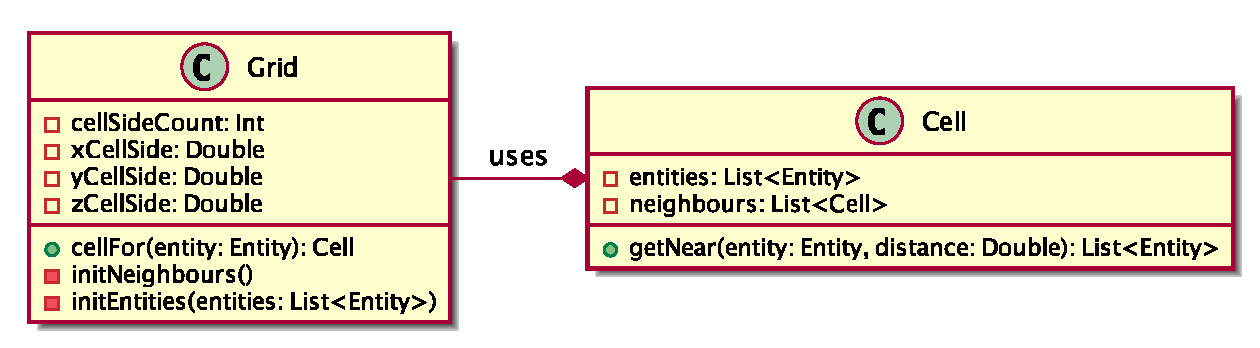
\includegraphics[width=0.8\textwidth]{../imgs/grid}
                \caption{Grilla}
                \label{fig:grid_implementation}
            \end{figure}

        \subsection{Entidades}

            Todos los agentes, no importa si son depredadores o no, son representados utilizando la clase \textit{Entity}. \\
            Cada entidad cuenta con las siguientes propiedades:
            \begin{itemize}
                \item id: Identificador de la entidad. Son únicos.
                \item type: Determina el tipo de la entidad.
                \item radius: Determina el radio de la entidad.
                \item position: Posición $(x, y, z)$ en el espacio.
                \item velocity: Velocidad $(v_x, v_y, v_z)$ en el espacio.
            \end{itemize}

            A su vez, cada \textit{Entity} cuenta con una manera de poder calcular la distancia (desde los bordes) a otra \textit{Entity} y de poder determinar si otra \textit{Entity} está en su rango de visión.

            \begin{figure}[H]
                \centering
                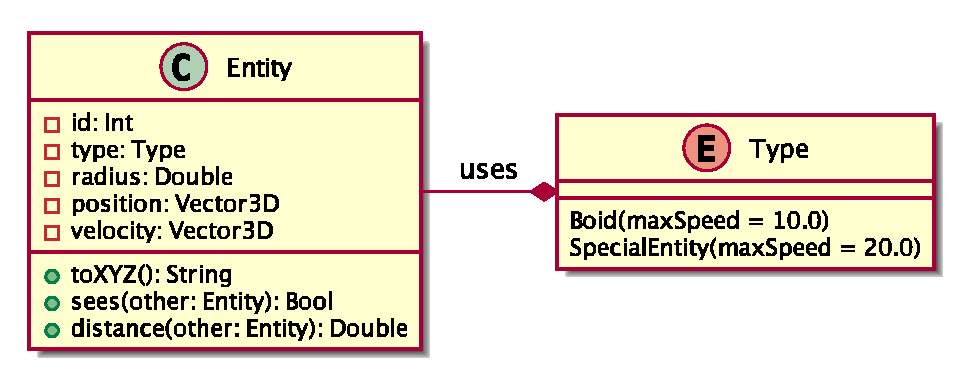
\includegraphics[width=0.5\textwidth]{../imgs/entity}
                \caption{Entidad}
                \label{fig:entity_implementation}
            \end{figure}

        \subsection{Reglas}
            Para la implementación de las reglas, se optó por tener una clase abstracta base \textit{Rule}, la cual cuenta con un factor que se le aplicará para aumentar o reducir su influencia. Tiene también un método público que es invocado por el algoritmo de simulación mediante el cual recibe todo lo necesario para que las implementaciones concretas puedan aplicarse.

            Cada implementación debe implementar los métodos:
            \begin{itemize}
                \item \textit{appliesTo}: Define a que tipos de entidades aplica la regla.
                \item \textit{doApply}: Aplica la regla y devuelve el ajuste de velocidad.
            \end{itemize}

            Existe otra clase abstracta llamada \textit{FlockRule} cuya finalidad es simplificar y agrupar aquellas reglas que apliquen únicamente para las entidades de tipo \textit{Boid}, ignorando al resto de las entidades. Sus implementaciones conforman al set básico de reglas propuesto por \textit{Reynolds}.
            \begin{figure}[H]
                \centering
                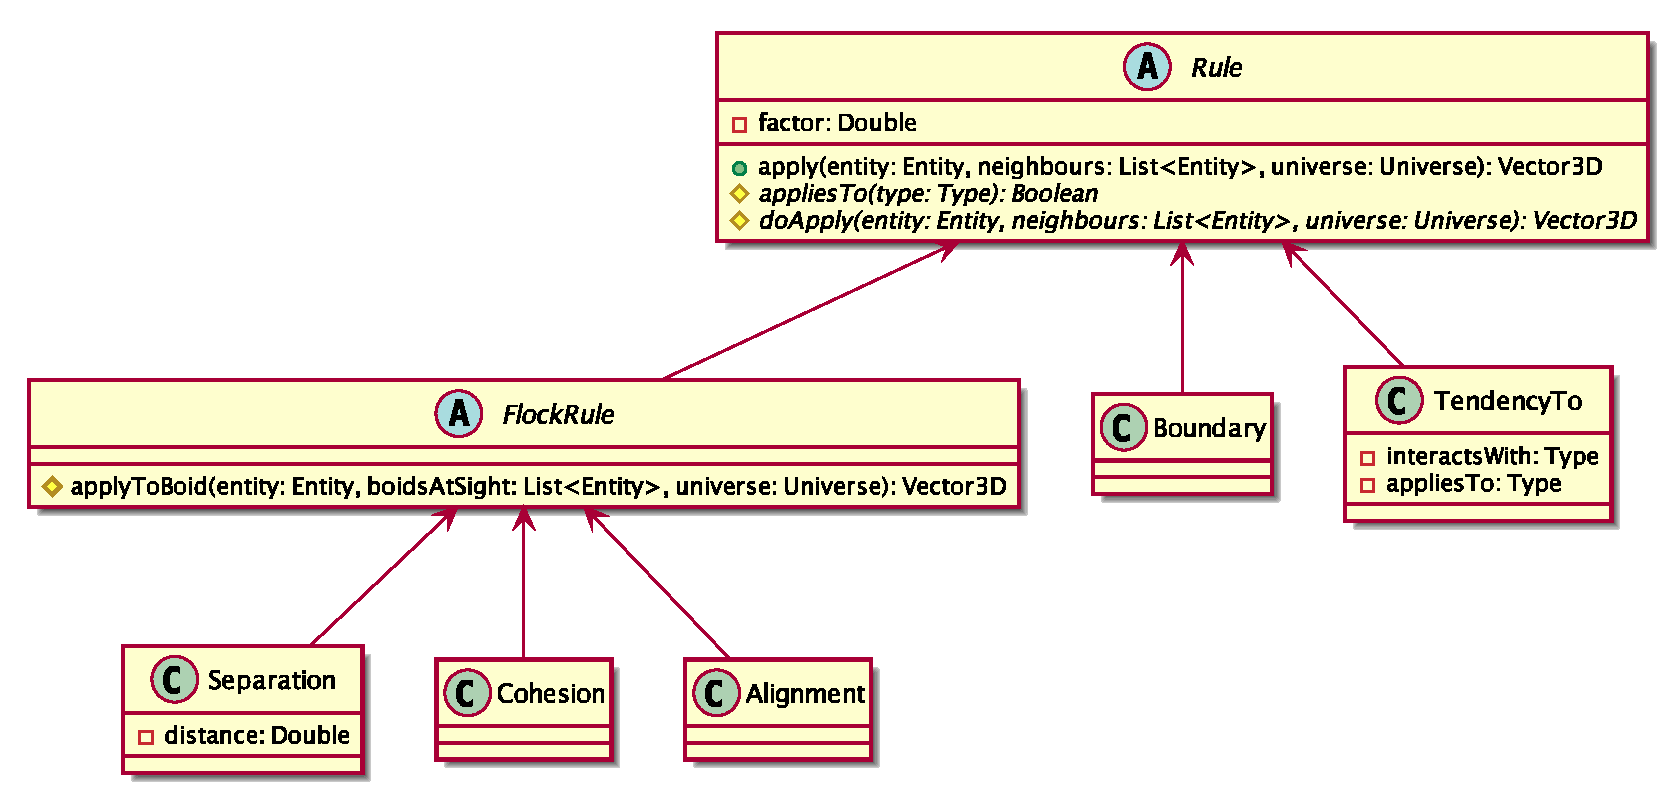
\includegraphics[width=0.8\textwidth]{../imgs/rules}
                \caption{Reglas}
                \label{fig:rules_implementation}
            \end{figure}
        \subsection{Simulación}

            \textit{Simulation} es la clase encargada de realizar la simulación.
            Internamente se ocupa de:
            \begin{itemize}
                \item Aplicar todas las reglas configuradas.
                \item Limitar la velocidad de todas las entidades ya que de ser únicamente por las reglas, la velocidad de cada \textit{Entity} tiende a aumentar.
                \item Mover aquellas entidades que se hayan escapado del universo en caso de haber condiciones de contorno.
            \end{itemize}

            \begin{figure}[H]
                \centering
                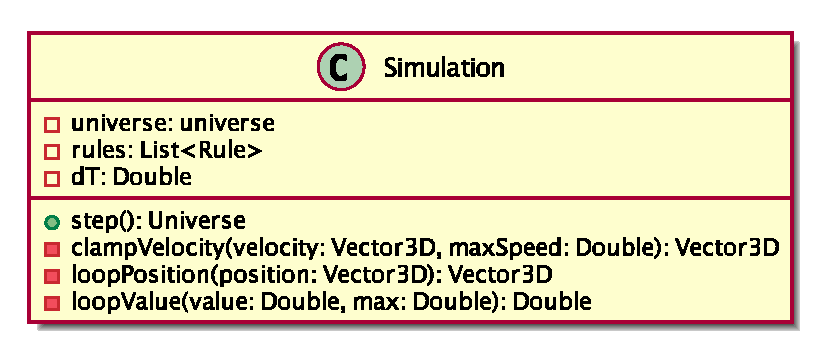
\includegraphics[width=0.5\textwidth]{../imgs/simulation}
                \caption{Simulación}
                \label{fig:simulation_implementation}
            \end{figure}

        \subsection{Optimizaciones}
            \subsubsection{Cálculo de vecinos}
                Para el cáclulo de vecinos se utiliza el método llamado \textit{Cell Index Method}. El mismo consiste en subdividir el espacio de simulación (Universo) en celdas de un determinado tamaño. Debido a que cada agente pertenece a una única celda, el método permite reducir el costo de búsqueda de vecinos de $N^2$ a un número más cercano a $N$. Dado que las dimensiones del universo son más de un orden de magnitud mayores que la distancia de búsqueda, se decidió fijar una cantidad de celdas determinadas para cada eje.

            \subsubsection{Cálculo de ángulo entre vectores}
                Se descubrió que el cáclulo del ángulo entre dos vectores era la operación que más tiempo demoraba, por lo que se implementó la función $acos$ propuesta por NVidia\cite{FastAcos}.

        \subsection{Visualización}
            Para realizar las animaciones y visualizaciones de las simulaciones se utiliza \textit{Ovito}.

            Para poder dar una idea de la posición en un espacio que cuenta con tres dimensiones, se decidió utilizar la posición de cada \textit{boid} para determinar el color que el mismo tendrá siguiendo las siguientes reglas:

            \begin{itemize}
                \item $R = 0.2 + (position.x / width) * 0.8$
                \item $G = 0.2 + (position.y / height) * 0.8$
                \item $B = 0.2 + (position.z / depth) * 0.8$
            \end{itemize}

            De esa manera, aquellos \textit{boids} que se encuentren en el mismo área de la simulación tendrán un color similar, lo que permite tener una idea de la distribución de las entidades dentro del universo.

    \section{Resultados}
        Si bien la implementación realizada soporta simular con o sin condiciones de contorno, se decidió que únicamente se analizarán escenarios con condiciones de contorno.

        A menos que se indique lo contrario, se utilizaron $10$ simulaciones para obtener los errores de cada gráfico.

        \subsection{Sin boids especiales}
            Para las simulaciones sin boids especiales, se estudia el comportamiento del sistema utilizando los siguientes parámetros:
            % \begin{center}
                \begin{table}[h]
                    \centering
                    \begin{tabular}{|r|l|}
                        \hline
                        Dimensión del universo & $32m$ x $32m$ x $32m$ \\
                        Condiciones de contorno & activadas \\
                        Número de boids & $1024$ \\
                        Número de especiales & $0$ \\
                        Distancia de interacción & $2m$ \\
                        Radio de boids & $0.1m$ \\
                        Velocidad máxima de boids & $32 m/s$ \\
                        Radio de especiales & $1.0m$ \\
                        Velocidad máxima de especiales & $64 m/s$ \\
                        \hline
                    \end{tabular}
                \end{table}
            % \end{center}

            Los factores de multiplicación base para cada una de las reglas son los siguientes:

            % \begin{center}
                \begin{table}[h]
                    \centering
                    \begin{tabular}{|r|l|}
                        \hline
                        Alineamiento & $0.25$ \\
                        Cohesión & $0.25$ \\
                        Separación & $0.25$ \\
                        Tendencia boid a especial & $-0.25$ \\
                        tendencia especial a boid & $0.25$ \\
                        \hline
                    \end{tabular}
                \end{table}
            % \end{center}

            \subsubsection{Polarización: Alineamiento}
                Se varía el factor de la regla de \textit{alineamiento} para ver su impacto en la polarización del sistema.

                \begin{figure}[H]
                    \centering
                    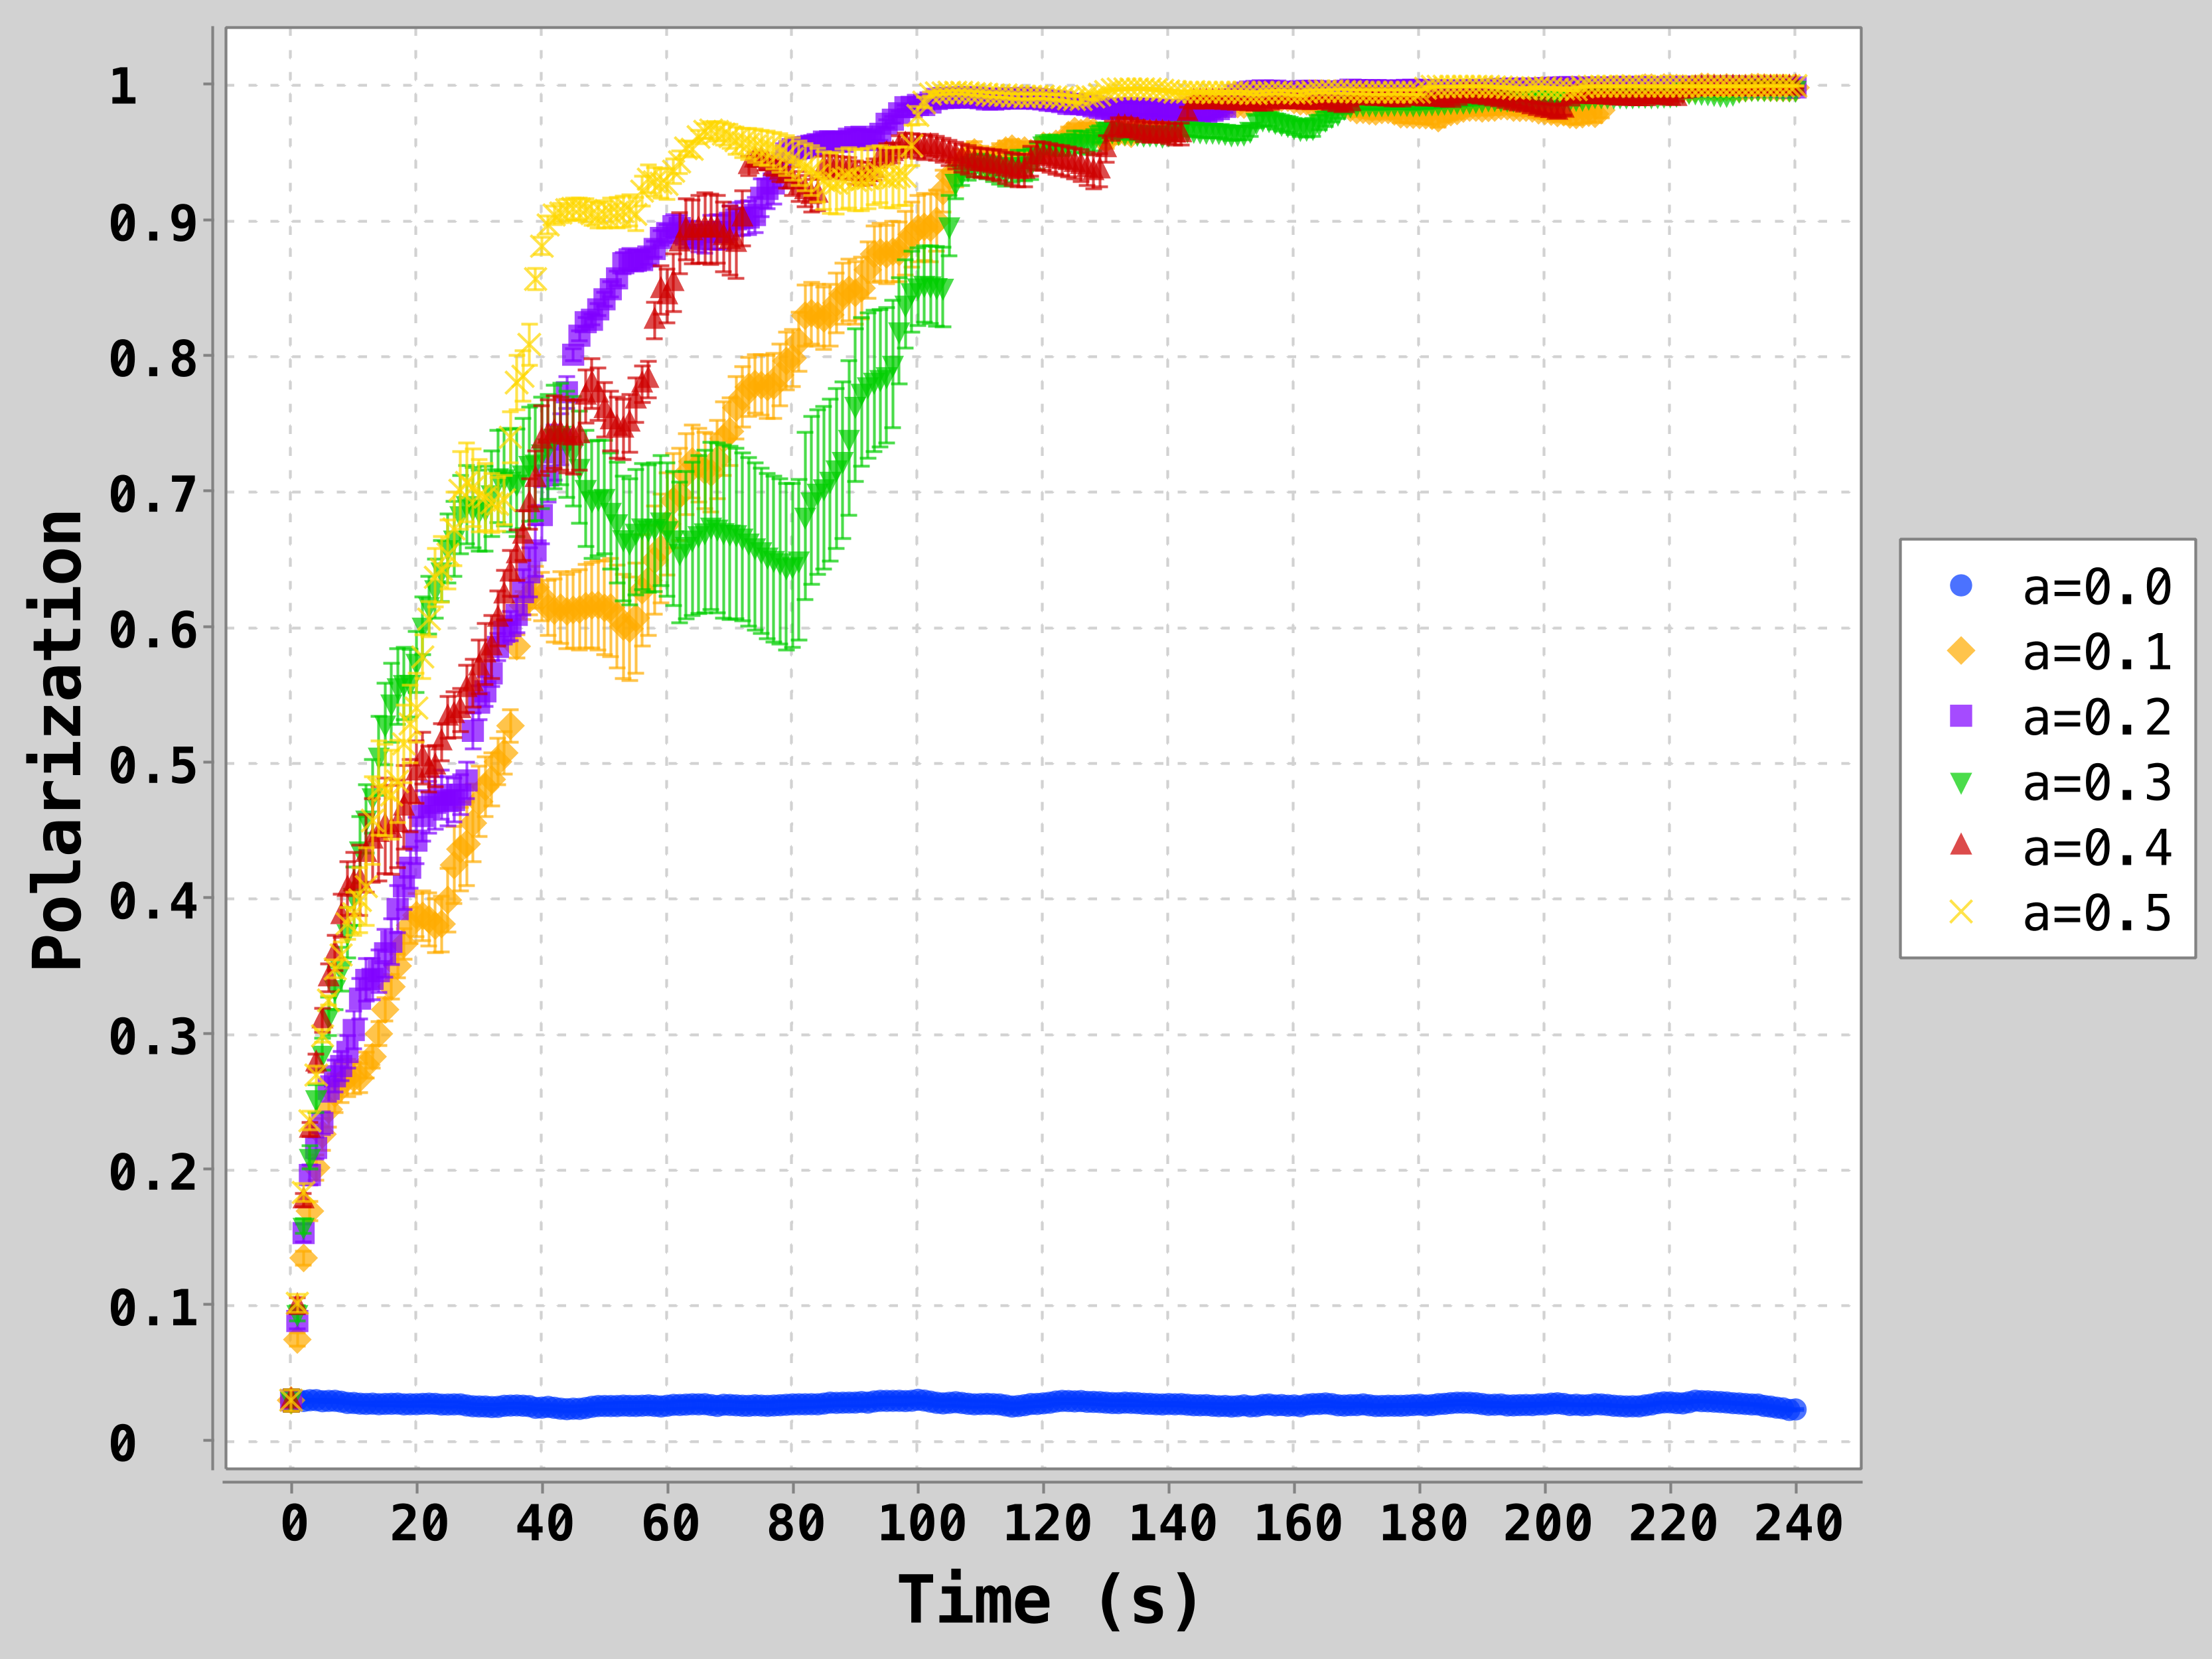
\includegraphics[width=0.8\linewidth]{{../imgs/polarization_a}.png}
                    \caption{Polarización variando factor alineamiento}
                    \label{fig:polarization_a}
                \end{figure}

                Se puede observar que variar el factor de la regla de \textit{polarización} tiene uno de dos resultados: Si el factor es $0$ (regla desactivada), el sistema se polariza; cualquier otro valor no afecta en mayor medida la rapidez con la que el sistema se polariza.

                \subsubsection{Polarización: Cohesión}
                Se varía el factor de la regla de \textit{cohesión} para ver su impacto en la polarización del sistema.

                \begin{figure}[H]
                    \centering
                    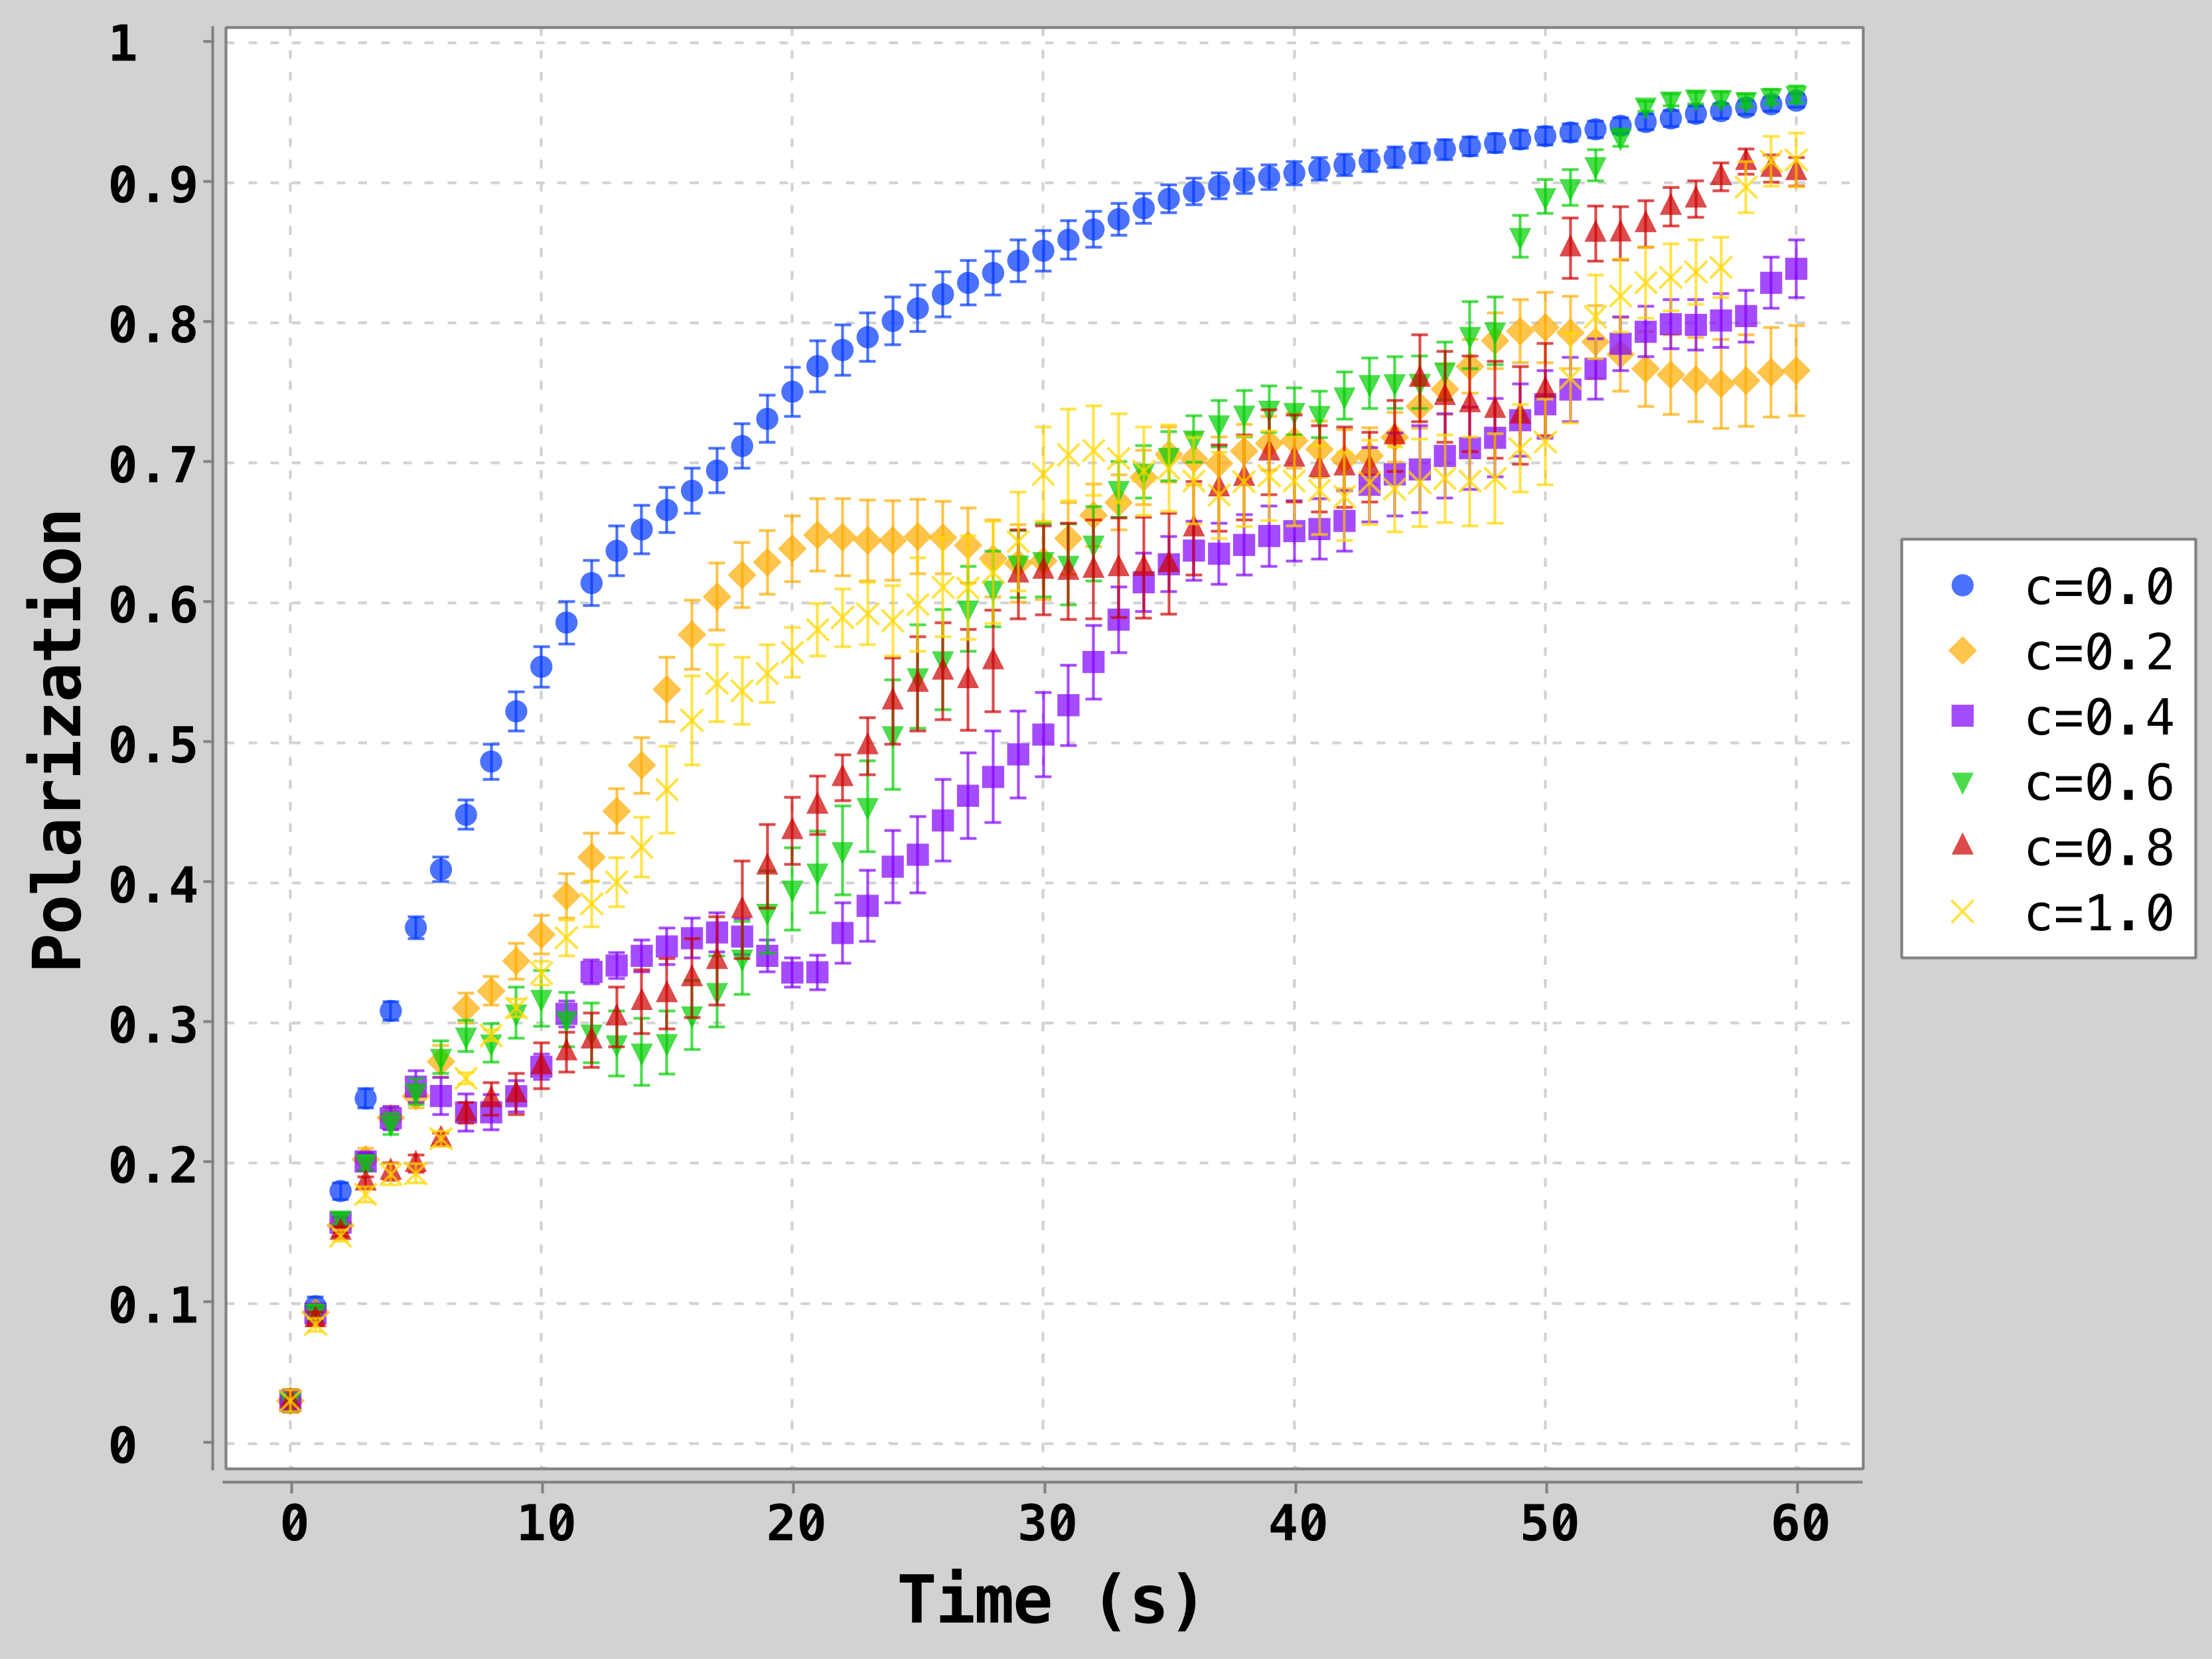
\includegraphics[width=0.8\linewidth]{{../imgs/polarization_c}.png}
                    \caption{Polarización variando factor cohesión}
                    \label{fig:polarization_c}
                \end{figure}

                Se puede observar que cuanto menos peso tenga la regla de polarización (factor tendiendo a cero), el sistema tiende a polarizarse con mayor rapidez, teniendo a la más rápida aquella que tiene la regla de \textit{cohesión} apagada.

                Ésto se genera ya que cada \textit{boid} no busca acercarse al centro de masa, por lo que como están las reglas de \textit{polarización} y \textit{separación} activadas, al estar cerca de otro \textit{boid} se alinea con el mismo.

                \subsubsection{Polarización: Separación}
                Se varía el factor de la regla de \textit{separación} para ver su impacto en la polarización del sistema.

                \begin{figure}[H]
                    \centering
                    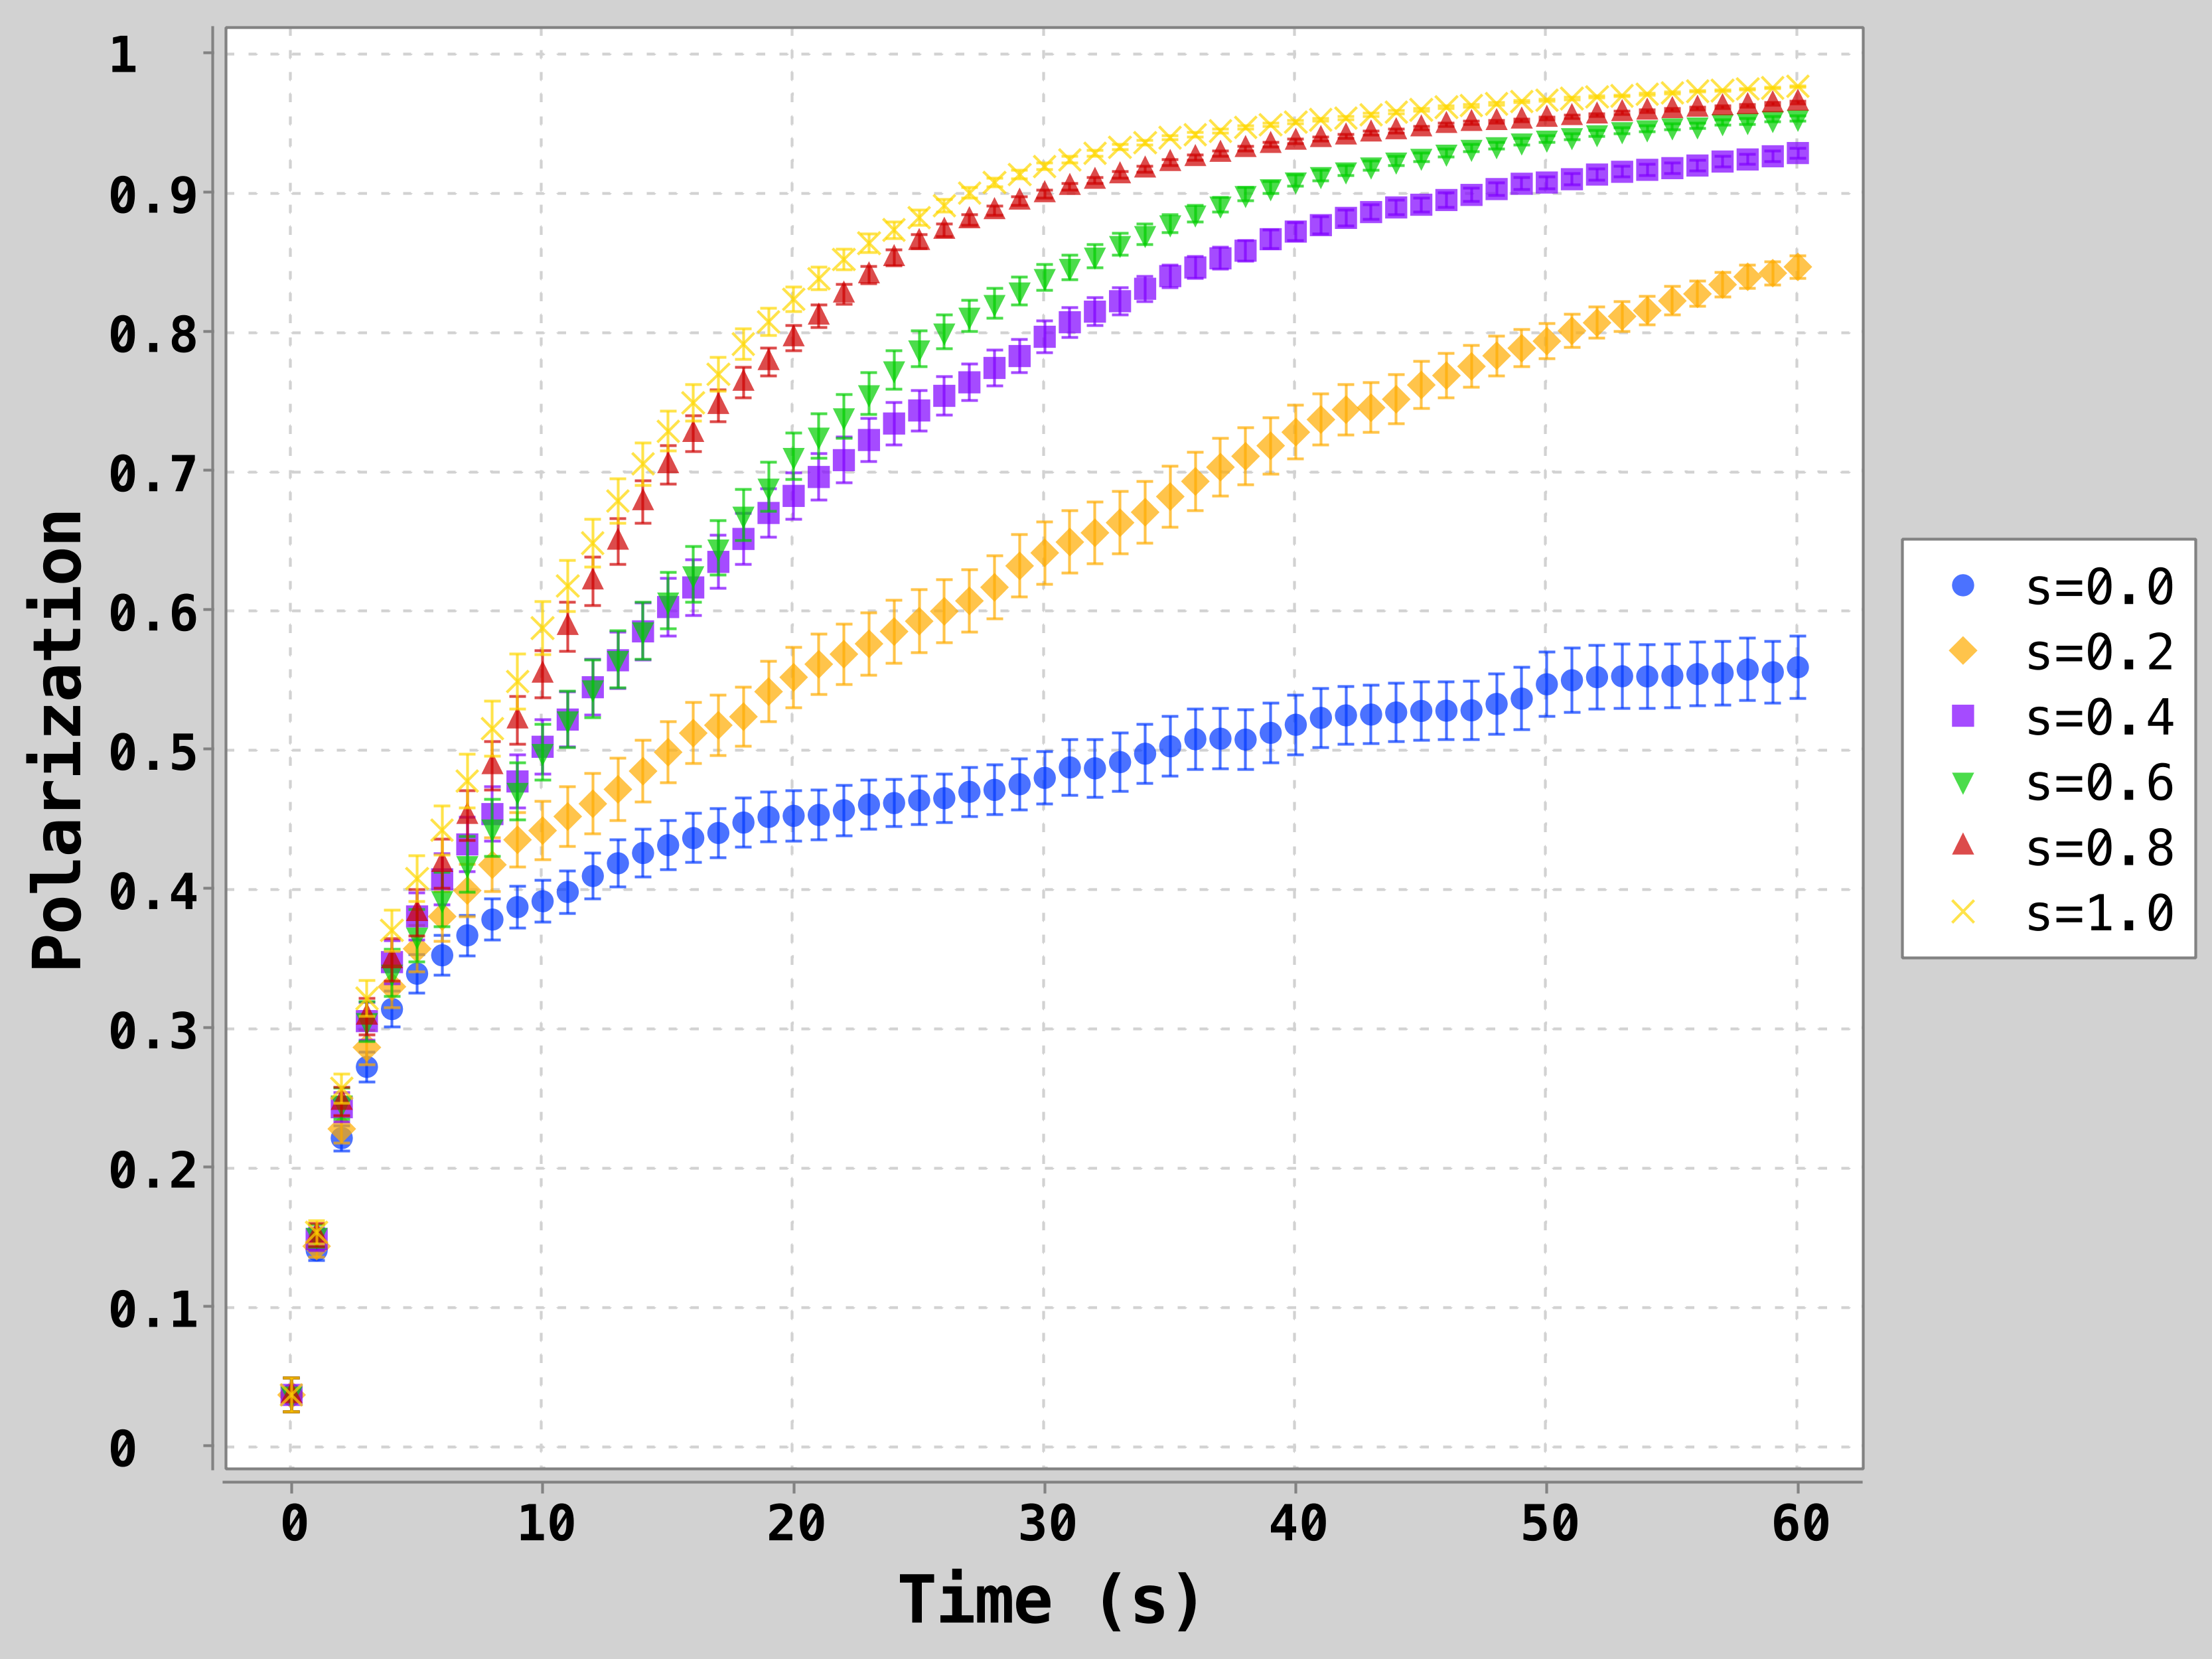
\includegraphics[width=0.8\linewidth]{{../imgs/polarization_s}.png}
                    \caption{Polarización variando factor separación}
                    \label{fig:polarization_s}
                \end{figure}

                Se puede observar que cuanto menos efecto tiene la regla de separación ($t \to 0$), más lento polariza el sistema.

                Ésto se debe a que, como cada \textit{boid} tiende a ir al centro de masa debido a la regla de \textit{cohesión},
                se termina generando una superposición de boids, por lo que el volúmen de influencia de esa bandada se reduce a un volúmen de influencia similar al de un único \textit{boid}
                y dado que el volúmen del universo es grande, la probabilidad de que dos boids se crucen es baja, por lo que toma más tiempo llegar a la polarización.

            \subsection{Con boids especiales}
                Se agregan $3$ boids especiales y se estudia la variación del factor de la regla "\textit{Tendencia a}".

                \begin{figure}[H]
                    \centering
                    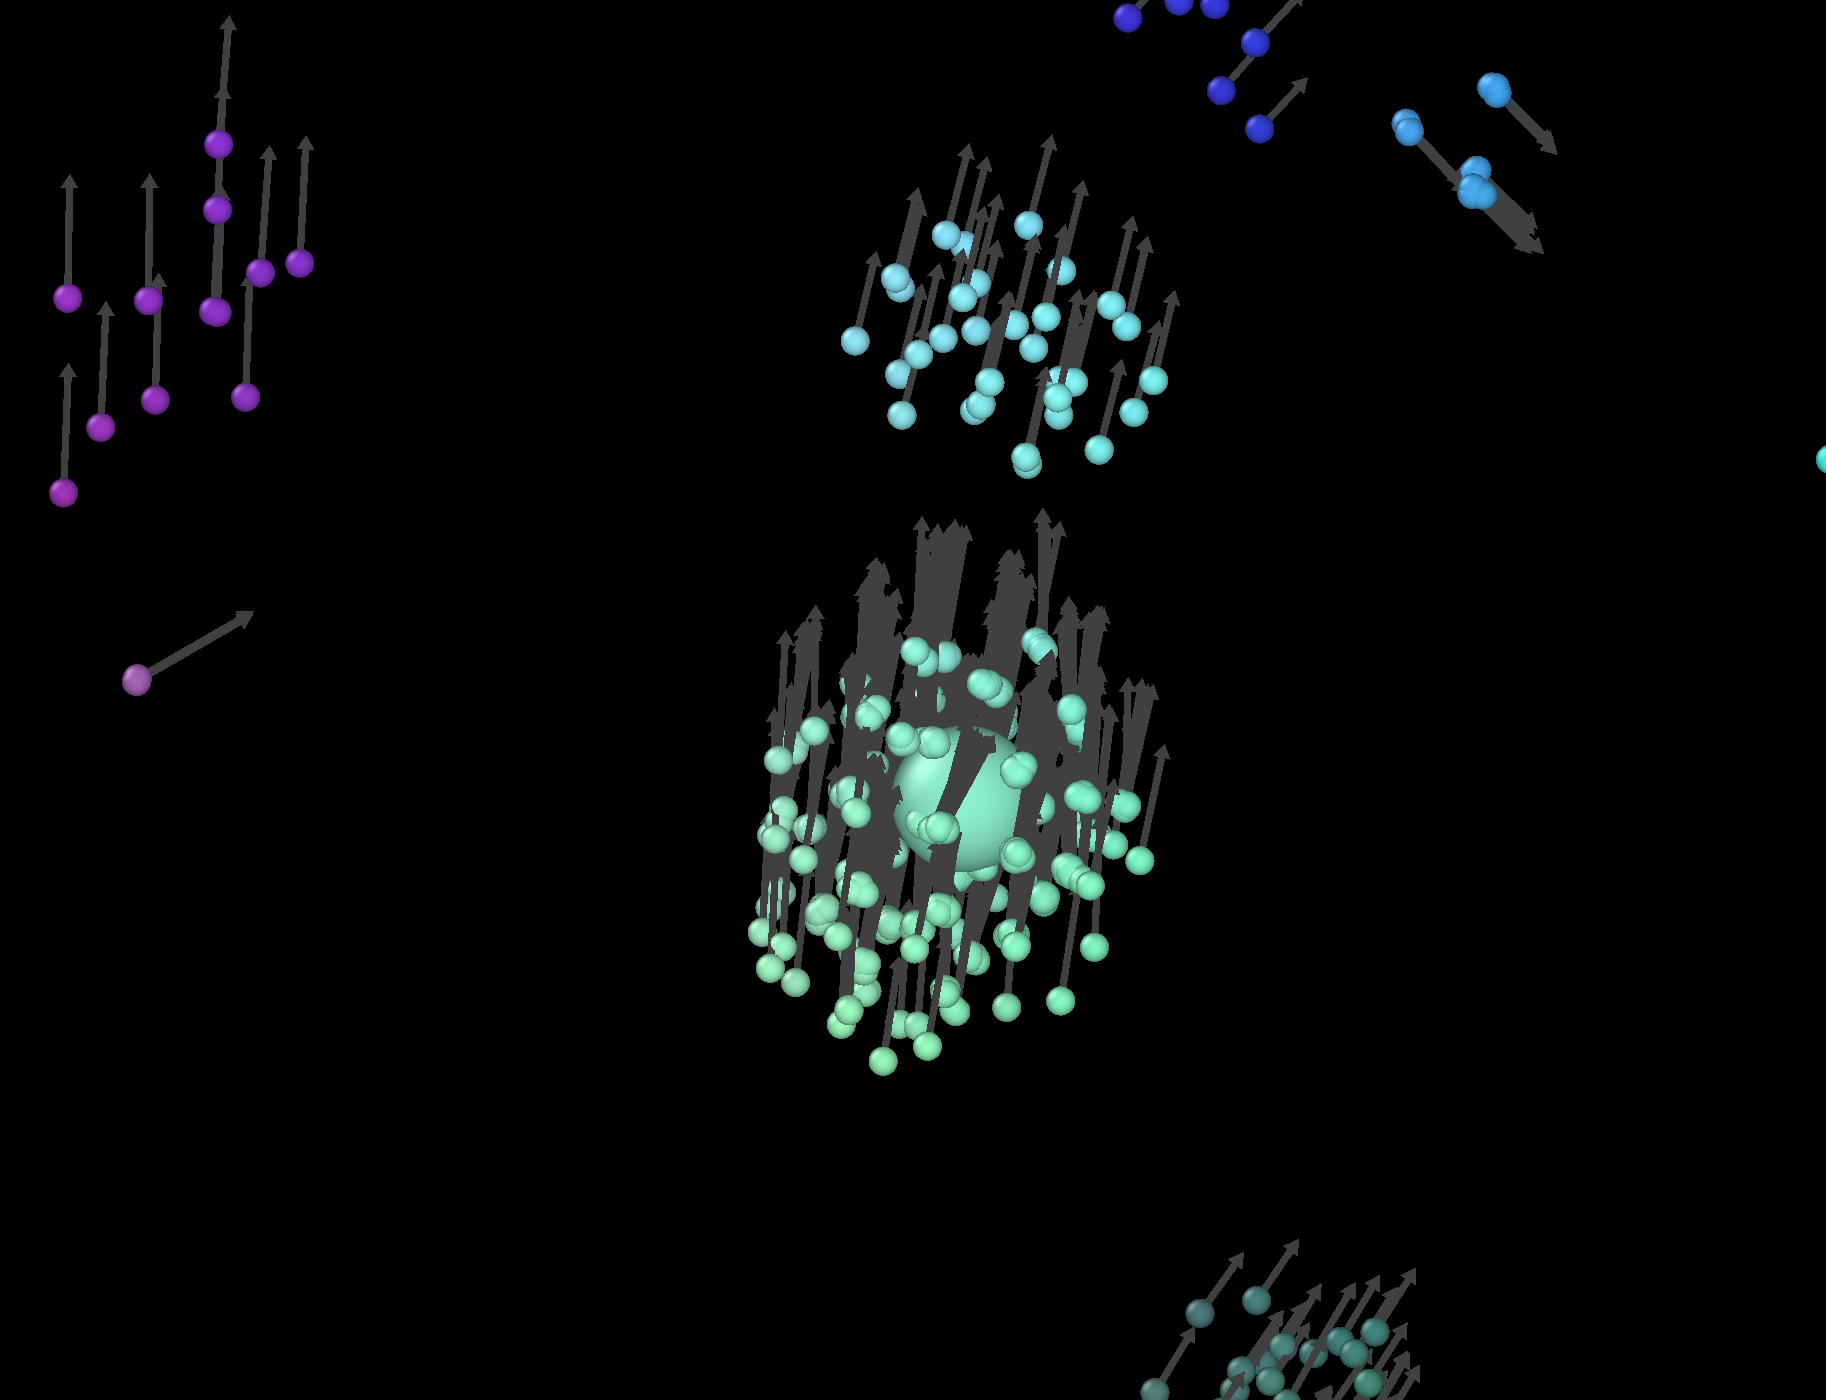
\includegraphics[width=0.8\linewidth]{{../imgs/tendency_to}.png}
                    \caption{Comportamiento: Tendencia a acercarse ($t > 0$)}
                    \label{fig:tendency_to}
                \end{figure}

                \begin{figure}[H]
                    \centering
                    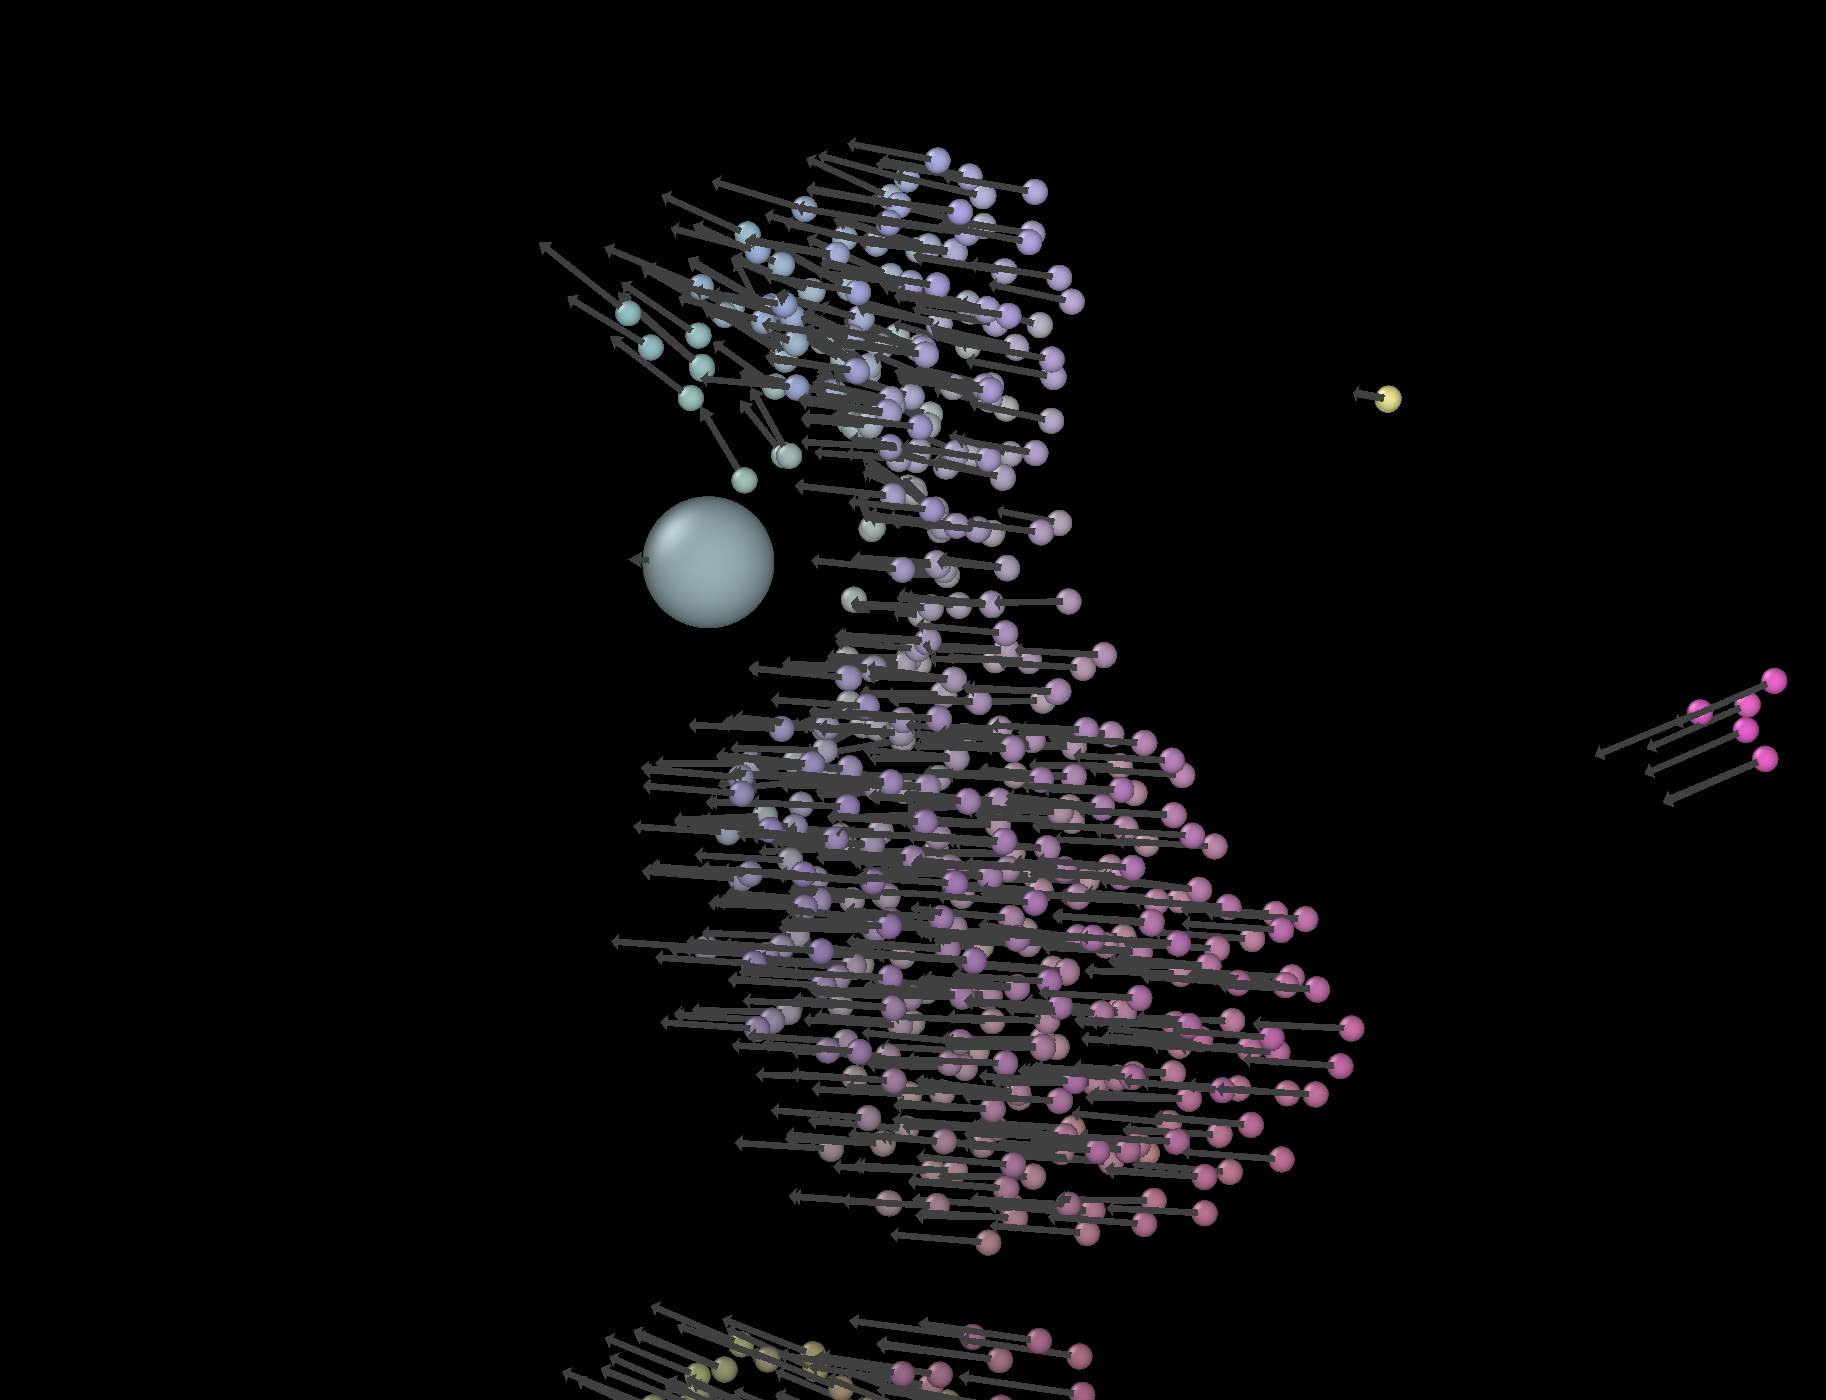
\includegraphics[width=0.8\linewidth]{{../imgs/tendency_away}.png}
                    \caption{Comportamiento: Tendencia a acercarse ($t < 0$)}
                    \label{fig:tendency_away}
                \end{figure}

                Se puede observar como afecta el signo del factor para la regla "\textit{Tendencia a}" el comportamiento de la bandada. Con $t > 0$ la bandada toma a la entidad especial como un líder de bandada, mientras que con $t < 0$, la bandada reacciona como si fuese un depredador.

                \begin{figure}[H]
                    \centering
                    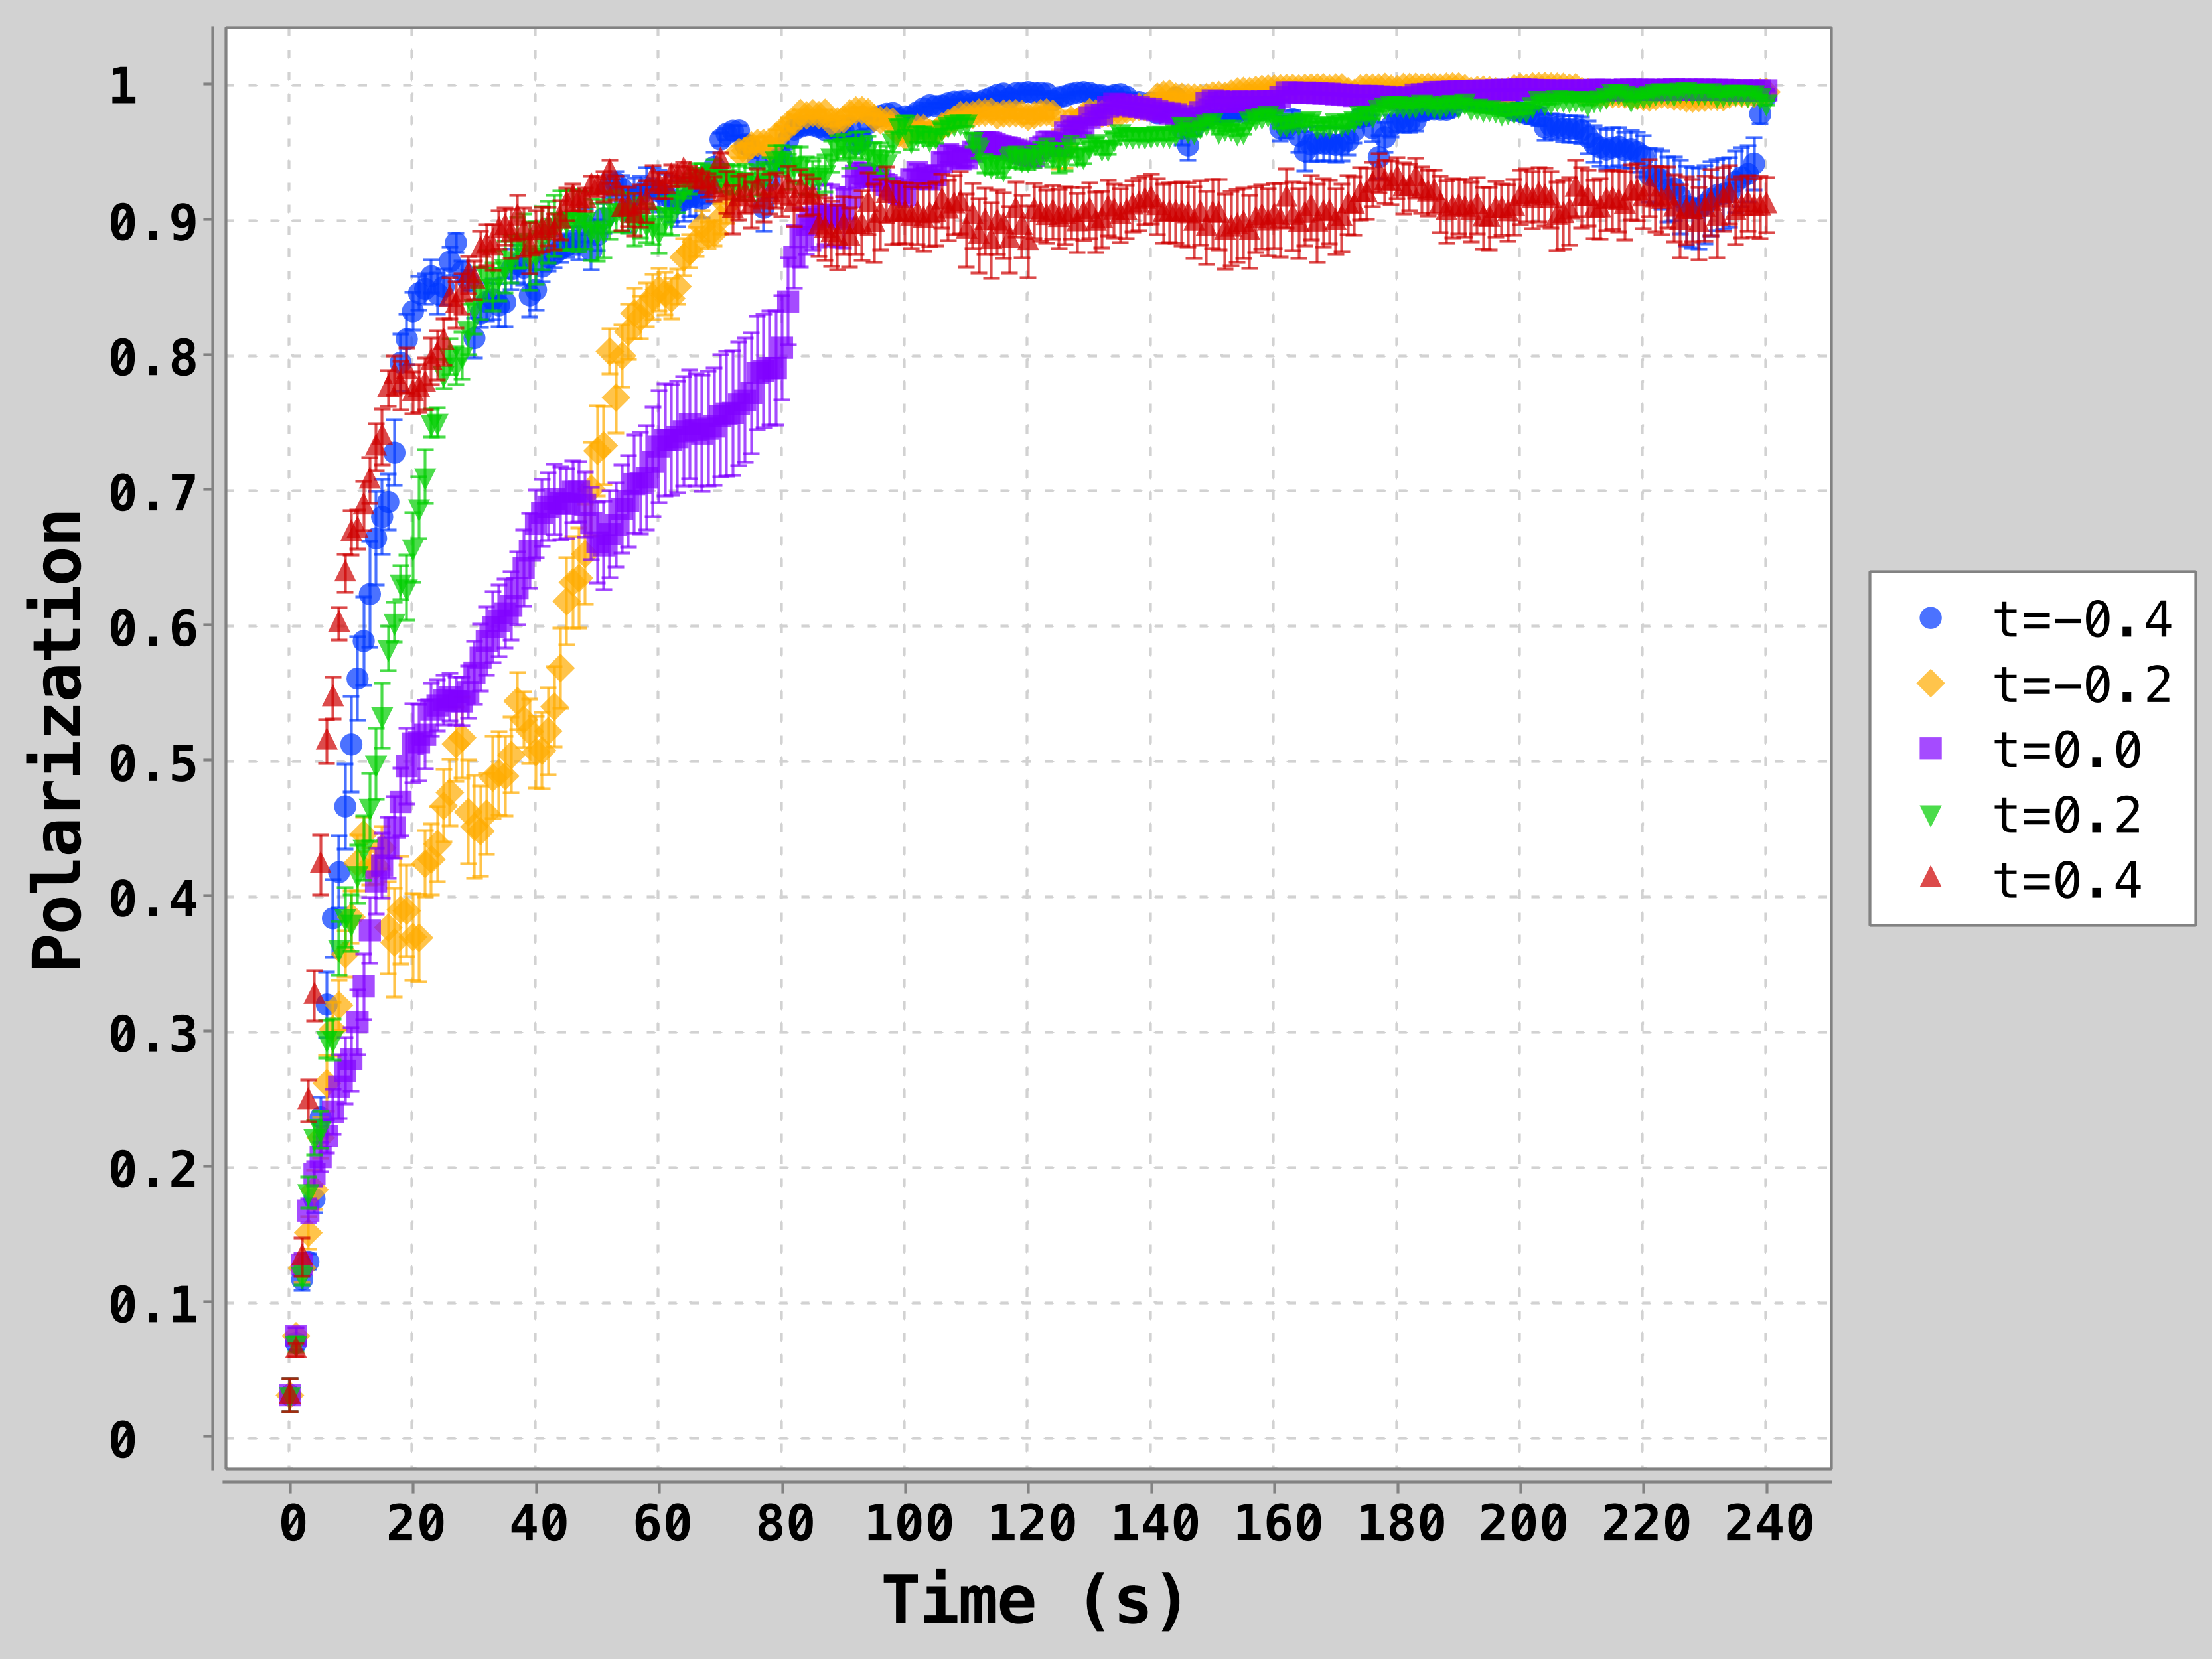
\includegraphics[width=0.8\linewidth]{{../imgs/polarization_t}.png}
                    \caption{Polarización: variando "Tendencia a"}
                    \label{fig:polarization_t}
                \end{figure}

                \begin{figure}[H]
                    \centering
                    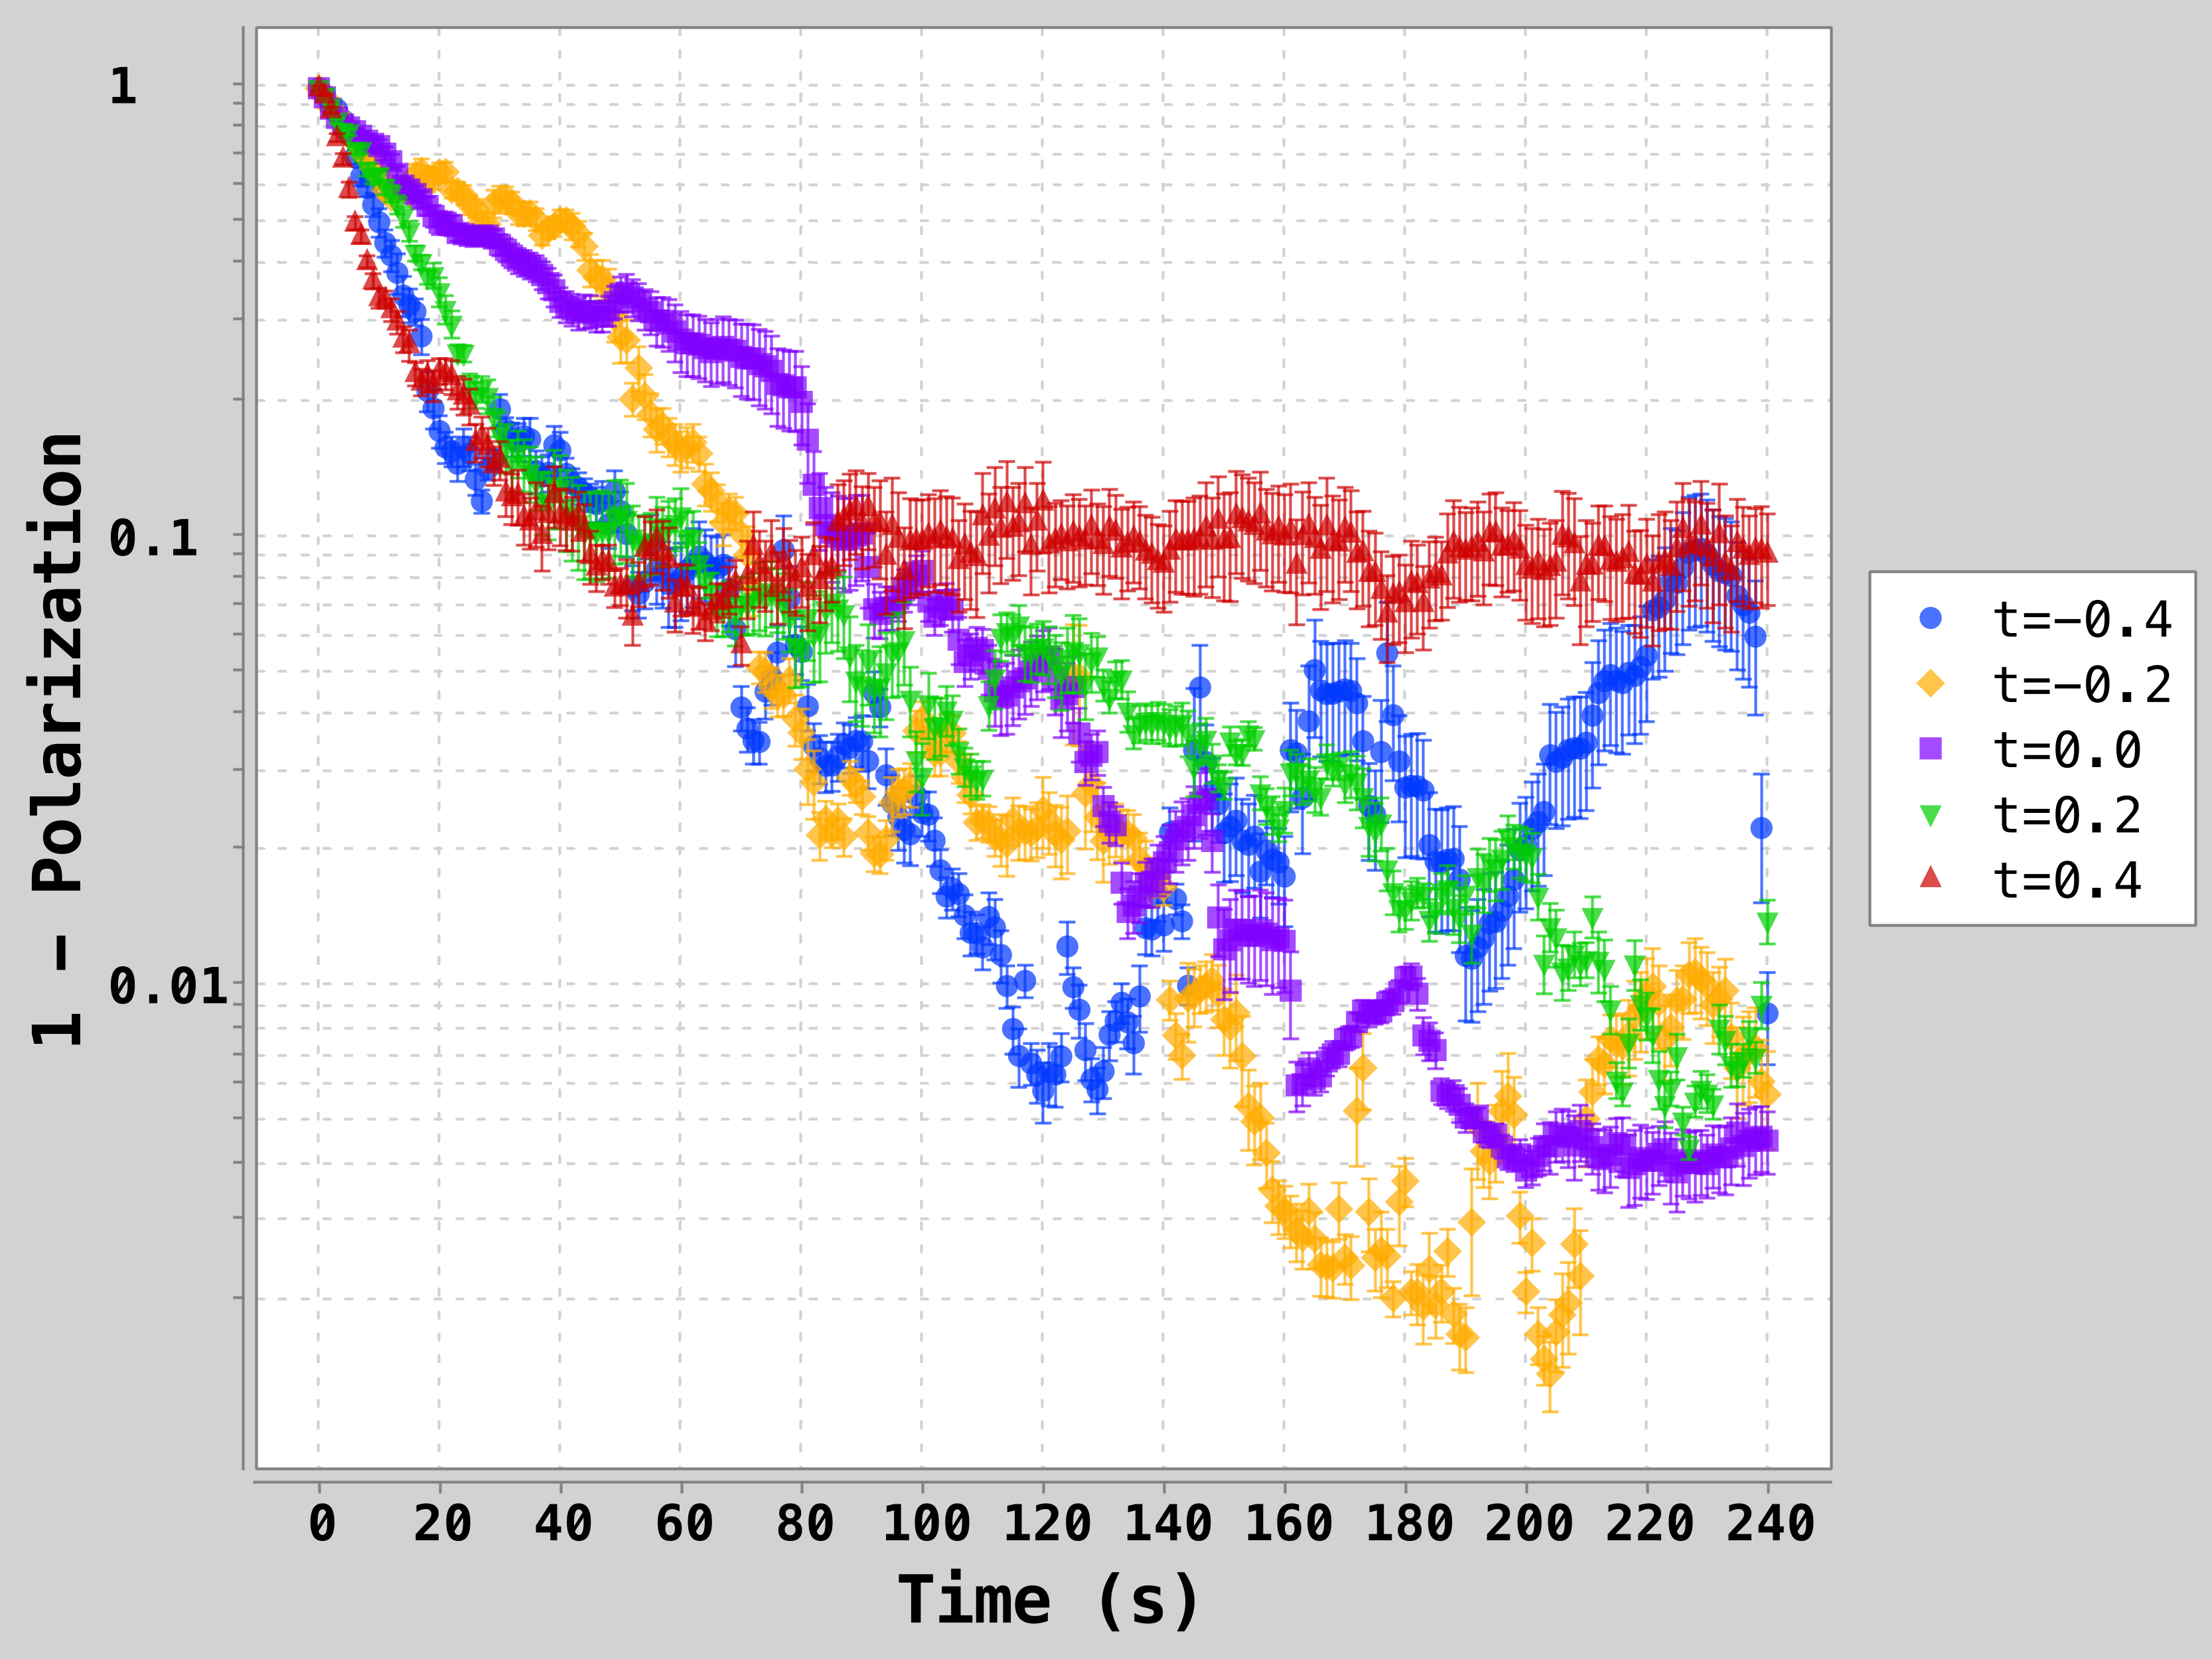
\includegraphics[width=0.8\linewidth]{{../imgs/polarization_t2}.png}
                    \caption{1 - Polarización: variando "Tendencia a"}
                    \label{fig:polarization_t2}
                \end{figure}

                Se puede observar que ambos extremos ($-0.4$ y $0.4$) en los que la regla de escapar o acercarse a los \textit{boids} especiales se encuentra con mayor intensidad son los que menos logran polarizar debido a las perturbaciones introducidas por éstas entidades nuevas.
                Con $t > 0$, se puede lograr una polarización del sistema similar a o mejor que sin la existencia de entidades especiales debido a el comportamiento de liderazgo que se genera. Mientras que con $t < 0$, es posible hacer que el sistema no llegue a polarizarse.

    \section{Conclusiones}
            Luego del análisis de los resultados, podemos concluir que a la hora de buscar una polarización más veloz del sistema basta con desactivar la regla de \textit{cohesión} para lograrlo.
            Sin embargo al hacerlo se pierde el comportamiento de bandada, haciendo que la simulación no pueda ser una buena representación de un sistema real.

            La regla de \textit{tendencia a} permite generar comportamientos complejos permitiendo simular líderes de bandada o depredadores dependiendo de qué signo se utilize en su factor.

            Por otro lado, la configuración de los parámetros iniciales de la simulación como así también los factores de las reglas cambian drásticamente el funcionamiento del sistema.
    \clearpage \printbibliography
\end{document}
